% !TeX spellcheck = de_DE_frami
%%%%%%%%%%%%%%%%%%%%%%%%%%%%%%%%%%%%%%%%%%%%%%%%
% COPYRIGHT: (C) 2012-2015 FAU FabLab and others
% Bearbeitungen ab 2015-02-20 fallen unter CC-BY-SA 3.0
% Sobald alle Mitautoren zugestimmt haben, steht die komplette Datei unter CC-BY-SA 3.0. Bis dahin ist der Lizenzstatus aller alten Bestandteile ungeklärt.
%%%%%%%%%%%%%%%%%%%%%%%%%%%%%%%%%%%%%%%%%%%%%%%%


\newcommand{\basedir}{fablab-document}
\documentclass{\basedir/fablab-document}

\usepackage{amssymb} % Symbole für Knöpfe
\usepackage{subfigure,caption}
\usepackage{eurosym}
\usepackage{textcomp} % \textcelsius
\usepackage{tabularx} % Tabellen mit bestimmtem Breitenverhältnis der Spalten
\usepackage{wrapfig} % Textumlauf um Bilder
\usepackage{float} % Ermöglicht H als Platzierungsoption
\renewcommand{\texteuro}{\euro}
\newcommand{\fachbegriff}[1]{(\textit{#1})}
\newcommand{\ts}[1]{\textsuperscript{#1}}
\newcommand{\ra}{$\Rightarrow$}

% \linespread{1.2}
% \fancyhead{}
\date{\today}
\author{kontakt@fablab.fau.de}
\title{Einweisung 3D-Drucker}

\begin{document}

\maketitle
\begin{center}
	Für die 3D-Drucker \textbf{Ultimaker\ts{2+}} und \textbf{Ultimaker\ts{3}}
\end{center}

\textbf{Nur eingewiesene Benutzer dürfen den Drucker selbstständig benutzen}, um teure Beschädigungen zu vermeiden. Wenn du noch nicht eingewiesen bist, frage eine:n Betreuer:in. Er erklärt dir die Bedienung und lässt dich unter Aufsicht dein gewünschtes Teil ausdrucken. Wenn du alles verstanden hast, darfst auch du dann die Einweisung unterschreiben und den Drucker in Zukunft selbstständig verwenden.

\section{Regeln und Hinweise}
% Hier sollte nur das wichtigste gegen "Kaputtmachen" des Druckers stehen.
Für die Benutzung ist es wichtig, dass du folgende Hinweise beachtest:

\begin{itemize}
 \item Obwohl das 3D-Drucken unter den Begriff ``Rapid Prototyping'' fällt, kann ein Druck je nach Größe und
 Präzision gut mehrere Stunden dauern. Betreuer:innen helfen dir, die Dauer abzuschätzen.
 \item Nicht unbeaufsichtigt drucken, immer wieder mal einen Blick darauf werfen, besonders am Anfang.\\
Wenn du nicht bis zum Ende deines Drucks da sein kannst, frage vorher einen Betreuer und hinterlasse einen Zettel mit Name und Kontaktdaten.
 \item Anleitung exakt beachten. Wenn du nicht weiter weißt oder dir unsicher bist, frag eine:n Betreuer:in.
 \item Verbrennungsgefahr an heißen Teilen:
  \begin{itemize}
   \item Extruder wird sehr heiß! Nicht direkt berühren, Vorsicht beim Abputzen.
   \item Bodenplatte der Ultimakers\ts2 wird sehr heiß. Erst abkühlen lassen und dann vorsichtig ohne zu berühren fühlen ob schon kalt genug.
  \end{itemize}
 \item Drucker ausschalten,
 \begin{itemize}
  \item wenn der Drucker groben Unfug oder sehr seltsame Geräusche macht
  \item wenn der Drucker nicht mehr benötigt wird
  \item Power-Switch befindet sich
  \begin{itemize}
   \item beim Ultimaker\ts{2+} hinten links am Gehäuse
   \item beim Ultimaker\ts{3} hinten rechts am Gehäuse
  \end{itemize}
 \end{itemize}
 \item \textbf{Keinen Schaber, Messer oder Ähnliches} verwenden, um Objekte von der Plattform zu lösen, denn dies kann die Glasplatte verkratzen
 \item am Drucker nichts von Hand bewegen ($\to$ \ref{manuelles-verfahren} Manuelles Verfahren auf Seite\, \pageref{manuelles-verfahren})
 \item Materialwechsel und sonstige Wartung darf nur gemeinsam mit einer Betreuerin/einem Betreuer durchgeführt werden.
 \item \textbf{Wiegen und Bezahlen nicht vergessen!}
\end{itemize}
\newpage

% % % % % % % % % % % % % % % %

\renewcommand{\contentsname}{Inhaltsverzeichnis / Arbeitsablauf}
\setcounter{tocdepth}{2}
\tableofcontents
\newpage

% % % % % % % % % % % % % % % %
\section{3D-Modell erstellen}
\subsection{Dateiformat}

Im STL-Dateiformat, Einheit: Millimeter. Alle gängigen 3D-Programme haben einen STL-Export.

\begin{itemize}
\item auf \href{https://thingiverse.com}{Thingiverse.com} gibt es viele vorgefertigte Modelle, als
Grundlage oder gleich zum fertig ausdrucken.
\item oder erstelle es mit einem Programm deiner Wahl
\begin{table}[H]
\centering
\begin{tabularx}{\textwidth}{|l|X|}
\hline \textbf{Name} & \textbf{Beschreibung} \\
\hline \multicolumn{2}{|c|}{\textit{kostenlose Software}}  \\
\hline Blender & relativ komplex aber auch für Freiformflächen geeignet  \\
\hline OpenSCAD & Skriptsprache für Konstruktion aus geometrischen Grundkörpern \\
\hline DesignSpark Mechanical & Angelehnt an professionelle CAD-Software, aber relativ einfach zu bedienen  \\
\hline TinkerCAD & sehr einfach, für Kinder gut geeignet  \\
\hline Google SketchUp & wenig Einarbeitung, geringer Funktionsumfang, für einfache Teile \\
\hline & \\
\hline \multicolumn{2}{|c|}{\textit{kostenpflichtige Software (proprietär)}}  \\
\hline PTC Creo, Solid Edge, Siemens NX & kostenlos beim RRZE für Studenten, professionelle Software \\
\hline Autocad Inventor & kostenlos bei Autodesk für Studenten ebenfalls für professionelle Anwendungen \\
\hline
\end{tabularx}
\end{table}
\item Die 3D-Daten müssen gewisse Regeln erfüllen. Bei Modellierungsprogrammen wie Blender ist etwas Vorsicht oder Nacharbeit nötig, die meisten Konstruktionsprogramme (Solid Edge und Konsorten, auch OpenSCAD) machen es prinzipbedingt von selber richtig. Zu den Einschränkungen bei Blender stehen am Ende der Anleitung noch weitere Informationen.
\end{itemize}

\subsection{Einschränkungen der Formen}
\begin{itemize}
\item \textbf{Maximale Abmessungen}
\begin{itemize}
 \item Ultimaker\ts{2+}: L:223 B:220 H:205mm
 \item Ultimaker\ts3:
 \begin{itemize}
   \item Nur linke oder rechte Düse: L:215 B:215 H:200mm
   \item Beide Düsen gleichzeitig: L:197 B:215 H:200mm
 \end{itemize}
 \item zur Sicherheit lieber ein paar Millimeter kleiner.
 \item Es ist in der Praxis meist nicht möglich, den Bauraum des Druckers auch nur annähernd auszunutzen! Wenn möglich, gestalte deine Objekte kleiner als 10x10x5cm (LxBxH).
\end{itemize}
\item \textbf{große Teile dauern ewig}, während des Drucks muss jemand dabei bleiben. Druckzeit für 30x30x30mm sind je
nach Präzision etwa 30-45 Minuten, ein größeres Volumen braucht entsprechend länger.
\item Durch das Druckverfahren sind gewisse Formen schlecht druckbar. Oft ist Ausprobieren angesagt.
\item Damit man auch \enquote{schwierige} Formen drucken kann, kann die Software \textbf{Stützstrukturen} erstellen. Wenn man dies erlaubt,
erzeugt der Drucker ein loses Geflecht unter Überhängen und Brücken,
das sich nach dem Ausdrucken mit einer Zange oder einem Skalpell entfernen lässt. So kann
man diese Begrenzungen umgehen. Nachteil ist die schlechtere
Oberflächenqualität und der Nachbereitungs-Aufwand.
\end{itemize}

\subsubsection{Drucken ohne Stützstruktur}
In diesem Abschnitt wird kurz beschrieben, welche Formen sich besonders gut drucken lassen, auch ohne Stützstruktur. Wenn es ohne großen Aufwand möglich ist, sollte man seine Konstruktionen gleich so wählen, dass sie gut druckbar sind.
\begin{center}
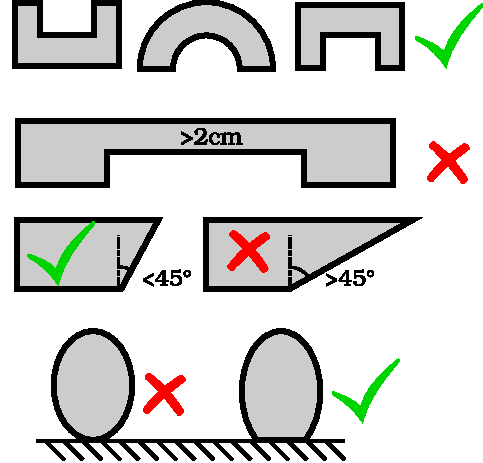
\includegraphics{./zeichnungen/formen.pdf}
\end{center}
\begin{itemize}
\item Überhänge sollten nicht zu groß sein
(Empfehlung {\textless}45\textcelsius{})
\item Brücken sollten nicht zu weit sein (Empfehlung {\textless}5mm)
\item Das Objekt sollte mit ausreichend großer Fläche plan auf dem Boden aufliegen
\item Der untere Teil des Objekts sollte immer eine stabile Unterlage für die darüberliegenden Schichten bilden. (Den Eiffelturm sollte man also nicht auf dem Kopf stehend drucken.)
\end{itemize}
\newpage

% % % % % % % % % % % %

\section{Vorbereitung}

\subsection{Putzen} \label{putzen}

Spätestens bei sichtbarem Schmutz (Staub o.Ä. auf der Plattform) oder bei schlechten Druckergebnissen

\begin{itemize}
 \item Bodenplatte mit Papiertuch und Oberflächenreiniger reinigen
 \item Extruderdüse ebenfalls mit Papiertuch reinigen
 \item \textbf{VORSICHT EVENTUELL HEISS!}
 \item Kunststoff(Filament)abfälle und leere Filamentspulen in die Sammelbox bei den Drucken
\end{itemize}

\subsection{Vorheizen}
Vorheizen ist nicht nötig, da es automatisch vor dem Druck geschieht.\\
\textbf{Im Gegenteil: Wenn der Extruder länger leersteht, brennt das Material fest!}

\subsection{Material}
Ich Fablab drucken wir ausschließlich mit  PLA. Andere Materialien können wir leider nicht anbieten.
\subsubsection{PLA}
\begin{itemize}
\item Organisches Material, Biokunststoff, nicht UV- und wetterbeständig
\item wird bei ca. 60\textcelsius{} weich
\item benötigt nicht zwingend ein beheiztes Bett es ist dennoch meist ratsam Das Druckbett auf ca. 60\textcelsius{} aufzuheizen. Das ist in Cura auch so voreingestellt.
\item Drucktemperatur beträgt meistens 210\textcelsius{}. Je nach Material kann sie allerdings ein wenig variieren.
\end{itemize}

PLA löst sich in Aceton(Dampf) auf.
%\todo{Beispielbild}

\subsection{Materialwechsel}
Wir haben verschiedene Materialfarben auf Lager. Wenn du eine andere möchtest, frag einfach nach.
Der Materialwechsel sollte aber \textbf{nur durch einen Betreuer:innen} erfolgen. (Infos für Betreuer:innen $\to$ \ref{filamentwechsel})

% % % % % % % % % % % %

\section{3D-Modell umwandeln und ausdrucken}

\subsection{Cura für Ultimaker (2\texttt{+} und 3)}
\begin{itemize}
\item In der oberen Leiste links den richtigen Drucker auswählen (Ultimaker Ultimaker\ts{2+} oder Ultimaker\ts3)
\item mit Klick auf das Ordnersymbol STL-Datei öffnen oder Datei einfach in das Cura-Fenster ziehen. So können auch mehrere Dateien hinzugefügt werden.
\item Objekt nach Wunsch auf eine spezifische Seite legen, skalieren, bewegen, drehen etc.
\item Sicherstellen dass in der oberen Leiste in der Mitte \enquote{Generic PLA} als Material ausgewählt ist
\item Obere Leiste auf der rechten Seite anklicken:
  \begin{itemize}
    \item Schichtdicke zwischen 0,06mm und 0,15mm (Ultimaker Ultimaker\ts{2+}) bzw. 0,2mm (Ultimaker\ts3) auswählen
    \item Infill einstellen: 20\% sind meistens ein recht guter Kompromiss aus materialersparnis und Stabilität
    \item ggf. ``Support`` (Stützstrukturen) und ''Adhesion``(zusätzliche Schürzze um Modell durcken für bessere Haftung) auswählen
    \item Unter \enquote{Customize} kann noch eine Vielzahl anderer Option eingestellt werden. Bitte Verändere die Einstellungen zur Drucktemperatur und Gescwindigkeit nicht bzw. nur nach Rücksprache mit einer Betreuerin/einem Betreuer.
  \end{itemize}
\item Solange die Daten umgerechnet werden, ist der Save-To-Disk/Removable-Knopf ausgegraut. Unter dem Knopf erscheint ein Fortschrittsbalken.
\item Über \enquote{Preview} kann man sich eine Vorschau der Druckbahnen inklusive Stützstruktur anzeigen lassen.
\item SD-Karte in den Kartenleser (Ultimaker\ts{2+}) oder USB-Stick (Ultimaker\ts3) einstecken
\item Save-To-Disk/Removable-Knopf klicken. Wenn der Knopf ausgegraut ist, warten, bis die Datei fertig gescliced wurde und dann nochmal klicken.
\item Wenn die Datei auf die Speicherkarte/den Stick gespeichert wurde, das Medium in Windows auswerfen und in den Drucker einstecken.
\end{itemize}

\section{Bezahlen und abschließen}

Um das Objekt von der Platte zu lösen vorsichtig arbeiten. Meistens lässt es sich von Hand lösen. Wenn nicht,
warten bis sich die Platte etwas abgekühlt hat. \textbf{Nicht versuchen, das Objekt mit scharfen oder spitzen Gegenständen herunter zu hebeln!}
Sollte das Tape oder die Folie auf der Plattform beim Herunterlösen kaputt gehen, bitte einen \textbf{Betreuer es zu erneuern}.

Drucker reinigen, siehe \ref{putzen}.

Objekt mit Feinwaage (steht meist bei den 3D-Druckern) abwiegen, Preis pro Gramm ist im Kassensystem eingetragen.

Es muss alles mitgewogen werden, auch die Stützstruktur und der Müll, den der Extruder anfangs ausspuckt. \textbf{Fehldrucke müssen ebenfalls bezahlt werden.}
\pagebreak

% % % % % % % % % % % %

\section{Zusatzinfos für Benutzer}

\subsection{Manuelles Verfahren}\label{manuelles-verfahren}
Manchmal muss man vor einem Druck, z.\,B. um die Plattform oder die Düse zu säubern, den Extruder bewegen.
Das darf bei beiden Druckern \textbf{nicht von Hand} gemacht werden!

% % % % % % % % % % % % % % %

\section{Infos für Experten}

\subsection{Kurze Einführung in die wichtigsten Fachbegriffe bei STL:}

\begin{itemize}
\item Einheit \fachbegriff{unit}: Länge, die der Zahl „1“ entsprechen soll (bei uns
1 Millimeter)
\item Punkt \fachbegriff{vertex}: Stelle im Raum
\item Kante \fachbegriff{edge}: Verbindungslinie zwischen zwei Punkten
\item Fläche \fachbegriff{face}: Dreieck, das zwischen drei Punkten bzw. zwei
benachbarten Kanten aufgespannt wird. Im verwendeten STL-Dateiformat
gibt es nur Dreiecksflächen. Krümmungen werden aus vielen
Dreiecksflächen angenähert.
\item Polygonnetz \fachbegriff{mesh}: Gesamtheit aller Flächen, die einen Körper
ergibt. Alles innerhalb des Netzes soll mit Kunststoff gefüllt werden,
alles außerhalb ist Luft.
\end{itemize}

\subsection{Einschränkungen bei Blender und manchen anderen Programmen} \label{lowlevel-einschraenkungen}

Das 3D-Modell muss gewisse Einschränkungen erfüllen, damit die Drucksoftware es versteht. Da man mit Tools wie Blender auch unsinnige Dinge bauen kann (Modelle mit Löchern, unlogische Dinge bei denen innen und außen nicht eindeutig ist), muss auf folgendes geachtet werden.
\begin{itemize}
\item Wasserdicht: Der Körper muss rundum geschlossen sein, er darf keine
Löcher aufweisen,  die Hülle muss ein zusammenhängendes Netz sein.
\item Polygonnetz \fachbegriff{mesh} schneidet sich nicht selbst: Verschiedene
Körper dürfen sich nicht überlappen. Sie müssen stattdessen zu einem
Körper vereinigt werden. In Blender geht dies zum Beispiel mit dem
Boolean Modifier.
\item Mannigfaltig \fachbegriff{manifold}: Dieser Begriff ist schwierig zu
beschreiben. Vereinfacht gesagt dürfen zu jeder Kante nur zwei Flächen
gehören. Es dürfen also zum Beispiel keine Flächen innerhalb eines
Körpers existieren.
\end{itemize}

% % % % % % % % % % % % % %

\section{Infos für Betreuer:innen}

\subsection{Filamentwechsel}\label{filamentwechsel}

\subsubsection{Ultimaker\ts{2+}}
\begin{itemize}
    \item ''Material'' \ra ''Change''; Anweisungen im Display beachten
    \item Drucker heizt vor und fährt dann das Filament zurück
    \item Filament hinten vorsichtig entnehmen; nicht verknoten oder brechen!
    \item neues Filament auf Spindel und ''Ready'' drücken
    \item neues Filament einführen bis Fördermotor zieht; aufpassen dass Filament sich nicht verknotet!
    \item ''Ready'' drücken; Drucker fährt Filament vor und extrudiert
    \item wenn er schön extrudiert, nochmal drücken und das eingelegte Filament wählen
\end{itemize}


\subsection{Ausrichten der Buildplate}

\subsubsection{Ultimaker\ts{2+}}
\begin{itemize}
\item Extruder reinigen, dass sich kein Rest zw. Buildplate und Extruder befindet
\item Assistent: ''maintenance'' \ra ''buildplate''
\item den Anweisungen auf dem Display befolgen
\item man muss mal mit dem Rad und den Steppern, mal manuell mit den Schrauben die Buildplate leveln (zuerst auf 1mm, dann mit einem Blatt Papier)
\end{itemize}


\subsection{Ultimaker 2\texttt{+} demontieren und putzen}
Lasse es dir vorher von jemand mit Ahnung zeigen! Nur durchführen wenn unbedingt nötig.

Die Düse bitte nicht mit einem Metallstück freistochern, da hierdurch nur die Oberfläche verkratzt wird und die Düse nur noch schlechter funktioniert. Es ist möglich, fest sitzenden Dreck mit einem Stück Filament durchzudrücken. Dazu nimmt man sich ein Stück Filament und drückt es mit ausreichend Kraft durch den heißen Extruder. Eine Kombizange hilft. Dabei nicht abrutschen oder den Extruderkopf überlasten.

Es kann allerdings auch sein, dass die Düse schlicht verschlissen ist und ausgetauscht werden sollte. Düsen haben in etwa eine Lebensdauer von 500-600 Druckstunden, danach kann man sie guten Gewissens austauschen.

\begin{itemize}
 \item Anleitung zum Wechseln Entfernen der Düse:\\
 \url{https://support.ultimaker.com/hc/en-us/article_attachments/360010318879/Change_the_nozzle_of_the_Ultimaker_2plus.pdf}
 \item Für den folgenden Schritt Handschuhe und Gesichtsschutz tragen, es dürfen keine anderen Leute im Lab-Hauptraum sein, weil Kunststoffspritzer herumfliegen! Fenster öffnen und Lüftung anschalten.
 \item Düse auf feuerfeste Unterlage (Steinplatte) auf der Werkbank legen, mit Heißluftpistole auf 600\textcelsius{} einige Minuten lang erwärmen.
 \item Düse mit Zange greifen und mit Druckluft durchpusten.
 \item So oft aufheizen und auspusten, bis man durchschauen kann.
 \item Düse wieder einbauen (Alublock festhalten, Drucker muss aufgeheizt sein!). Dabei nur ganz schwach festschrauben.
\end{itemize}

\subsection{Ultimaker 3\texttt{+} demontieren und putzen}

\textbf{ACHTUNG: Beim Ultimaker 3 kann die Düse nicht einzeln gewecheselt werden. Hier müssen die ganzen Printcores getauscht werden: \url{https://support.ultimaker.com/hc/en-us/articles/360011580799-Changing-materials-and-print-cores-on-the-Ultimaker-3}}


\subsection{Pflege \& Wartung}

\begin{itemize}
\item Achsen müssen regelmäßig geölt werden (1x wöchentlich)
\item Riemenspannung und Riemenzustand überprüfen (leicht gespannt)\\
Ultimaker: \url{https://www.youtube.com/watch?v=grHmmmSoOfc}
\item die Ausrichtung und den Zustand der Buildplate überprüfen
\item die Düse außen putzen und auf Verstopfung untersuchen
\item lose herumhängende Kabel befestigen
\item Extruder-Coldend zerlegen und putzen (Filament-Abrieb, Förderwalze zugesetzt)
\item Extruder-Hotend begutachten und nur wenn unbedingt nötig zerlegen (Temperatursensorkabel ist sehr empfindlich)
\end{itemize}

\subsection{Firmwareupdates}

\begin{itemize}
\item den Drucker über USB mit dem Rechner verbinden
\item Cura zum Updaten verwenden
\end{itemize}

\subsection{Ultimaker-App}

Einige gute Hinweise mit Bildern zum Thema Druckerwartung bei Ultimaker-Druckern gibt es auch in der Ultimaker-App.
Darin enthalten ist auch eine Liste von oft gestellten Fragen zum Lösen von Fehlern.
Die Anwendung ist für iOS und Android erhältlich: \url{https://ultimaker.com/en/products/ultimaker-app}.
\ccLicense{3d-drucker-einweisung}{Einweisung 3D-Drucker}

\end{document}
